\section{Modellierung} % (fold)
\label{sec:modellierung}

\subsection{Ereignisgesteuerte Prozessketten} % (fold)
\label{sub:ereignisgesteuerte_prozessketten}

Aus der Aufgabenbeschreibung ergeben sich die in Abbildung~\ref{fig:epk} dargestellten Prozessketten für Erzeuger und Verbraucher. Hierbei ist zu erkennen, dass sich die Prozesse bei identischem Ablaufschema lediglich in den  durchgeführten Prüfungen und Operationen unterscheiden. Hierdurch liegt es nahe, dass die Ablaufsteuerung im objektorientierten Entwurf in einer abstrakten Basisklasse modelliert wird, und nur die unterschiedlichen Handlungen in den jeweiligen spezialisierten Ableitungen konkretisiert werden.

\begin{figure}[H]
\begin{center}
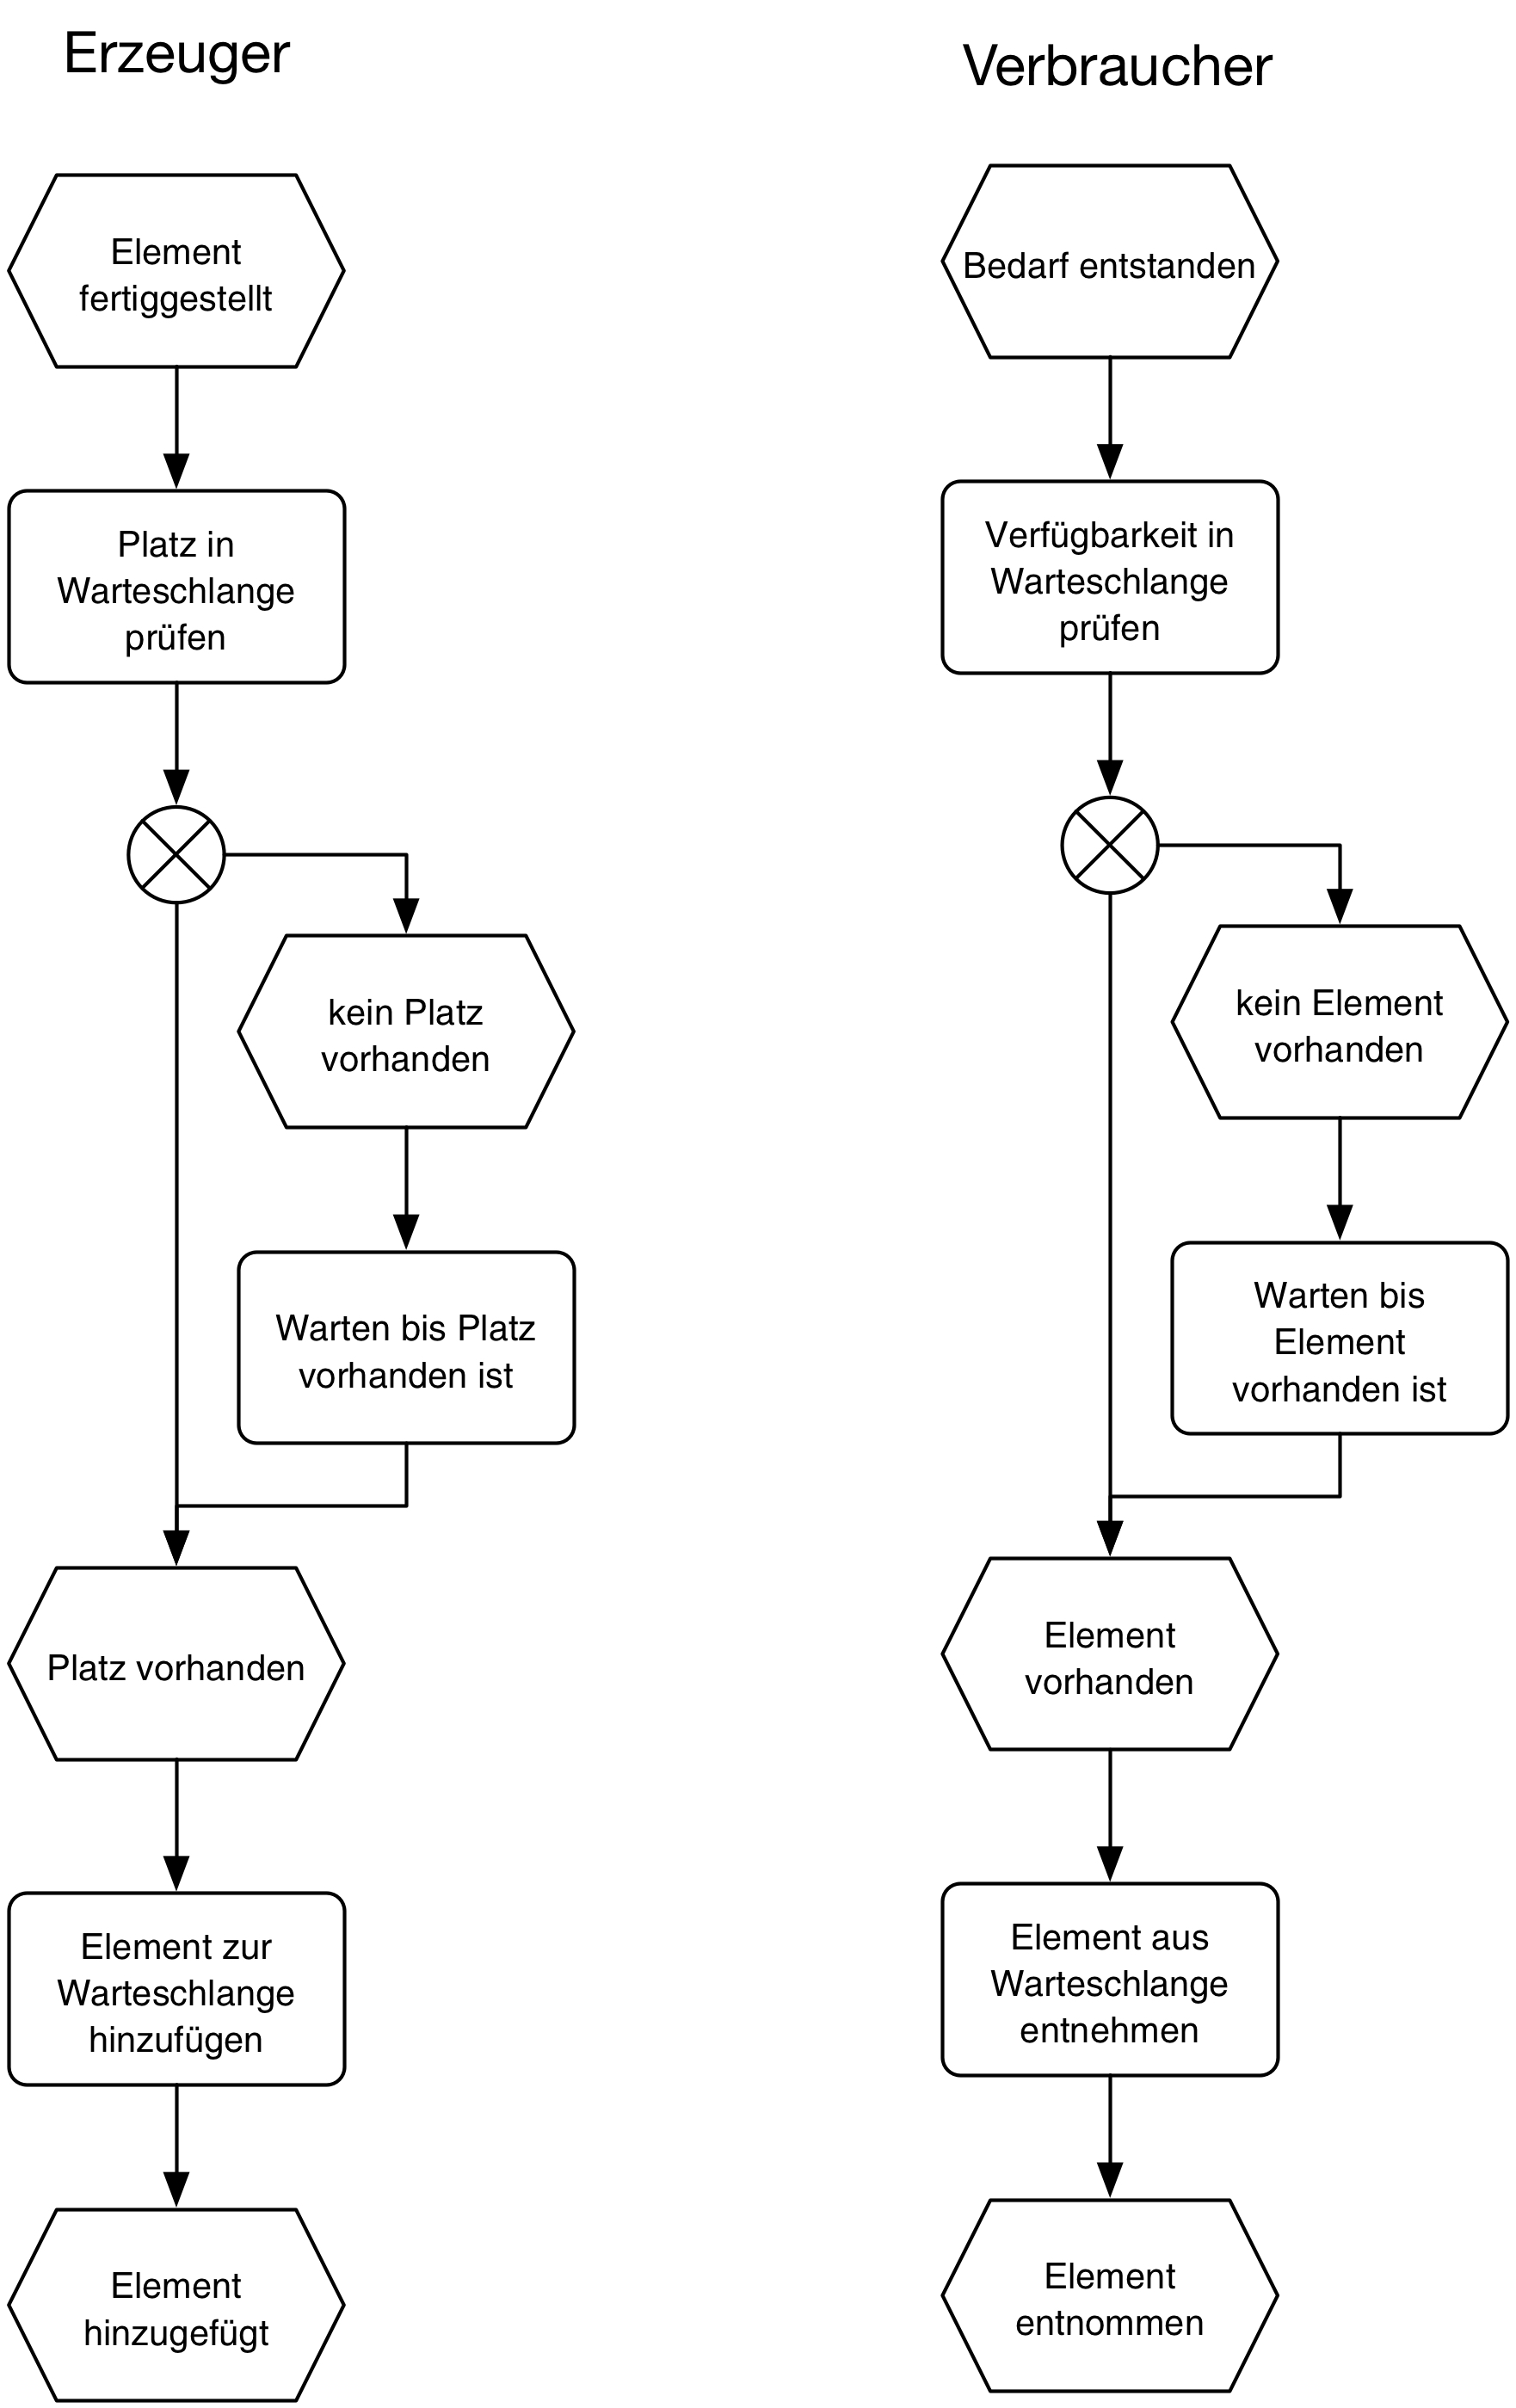
\includegraphics[width=.5\textwidth]{Erzeuger-Verbraucher-EPK.jpg}
\caption{Ereignisgesteuerte Prozessketten}
\label{fig:epk}
\end{center}
\end{figure}

% subsection ereignisgesteuerte_prozessketten (end)
% section modellierung (end)

\section{Implementierung} % (fold)
\label{sec:implementierung}

\subsection{Klasse: Akteur} % (fold)
\label{sub:klasse_akteur}

% subsection klasse_akteur (end)

\subsection{Klasse: Erzeuger} % (fold)
\label{sub:klasse_erzeuger}

% subsection klasse_erzeuger (end)

\subsection{Klasse: Verbraucher} % (fold)
\label{sub:klasse_verbraucher}

% subsection klasse_verbraucher (end)

\subsection{Klasse: Logger} % (fold)
\label{sub:klasse_logger}

% subsection klasse_logger (end)

\subsection{Sonstige Programmmerkmale} % (fold)
\label{sub:sonstige_programmmerkmale}

% subsection sonstige_programmmerkmale (end)
% section implementierung (end)

\newpage
\section{Laufzeitbetrachtungen} % (fold)
\label{sec:laufzeitbetrachtungen}

\subsection{Erzeuger schneller als Verbraucher} % (fold)
\label{sub:erzeuger_schneller_als_verbraucher}

% subsection erzeuger_schneller_als_verbraucher (end)

\subsection{Erzeuger langsamer als Verbraucher} % (fold)
\label{sub:erzeuger_langsamer_als_verbraucher}

% subsection erzeuger_langsamer_als_verbraucher (end)

\subsection{Ezeuger und Verbraucher gleich schnell} % (fold)
\label{sub:ezeuger_und_verbraucher_gleich_schnell}

% subsection ezeuger_und_verbraucher_gleich_schnell (end)

\subsection{Reduzierung auf einen Erzeuger und einen Verbraucher} % (fold)
\label{sub:reduzierung_auf_einen_erzeuger_und_einen_verbraucher}

Facade–Designpattern: Die n Verbraucher mit zufälligen Wartezeiten verhalten sich wie 1 Verbraucher mit kürzeren, aber ebenfalls zufälligen Wartezeiten. Dadurch ist die Anzahl der Verbraucher und analog dazu auch die der Erzeuger für die Betrachtung irrelevant.

% subsection reduzierung_auf_einen_erzeuger_und_einen_verbraucher (end)

% section laufzeitbetrachtungen (end)